\subsubsection{Test di Integrazione}
Con questa tipologia di test si vuole determinare il corretto funzionamento delle componenti progettate durante la definizione dell'architettura ad alto livello.

I test di integrazione saranno descritti nel modo seguente:
\begin{center}
\textbf{TI}[\textit{IdComponente}]
\end{center}
dove:
\begin{itemize}
\item
\textbf{IdComponente} rappresenta il codice identificativo crescente del componente considerato.
\end{itemize}
È stato scelto di utilizzare un approccio top-down nel determinare i test di integrazione. Di seguito viene riportato un diagramma informale per rendere chiara la struttura dei test identificati.
\begin{figure}[ht]
	\centering
	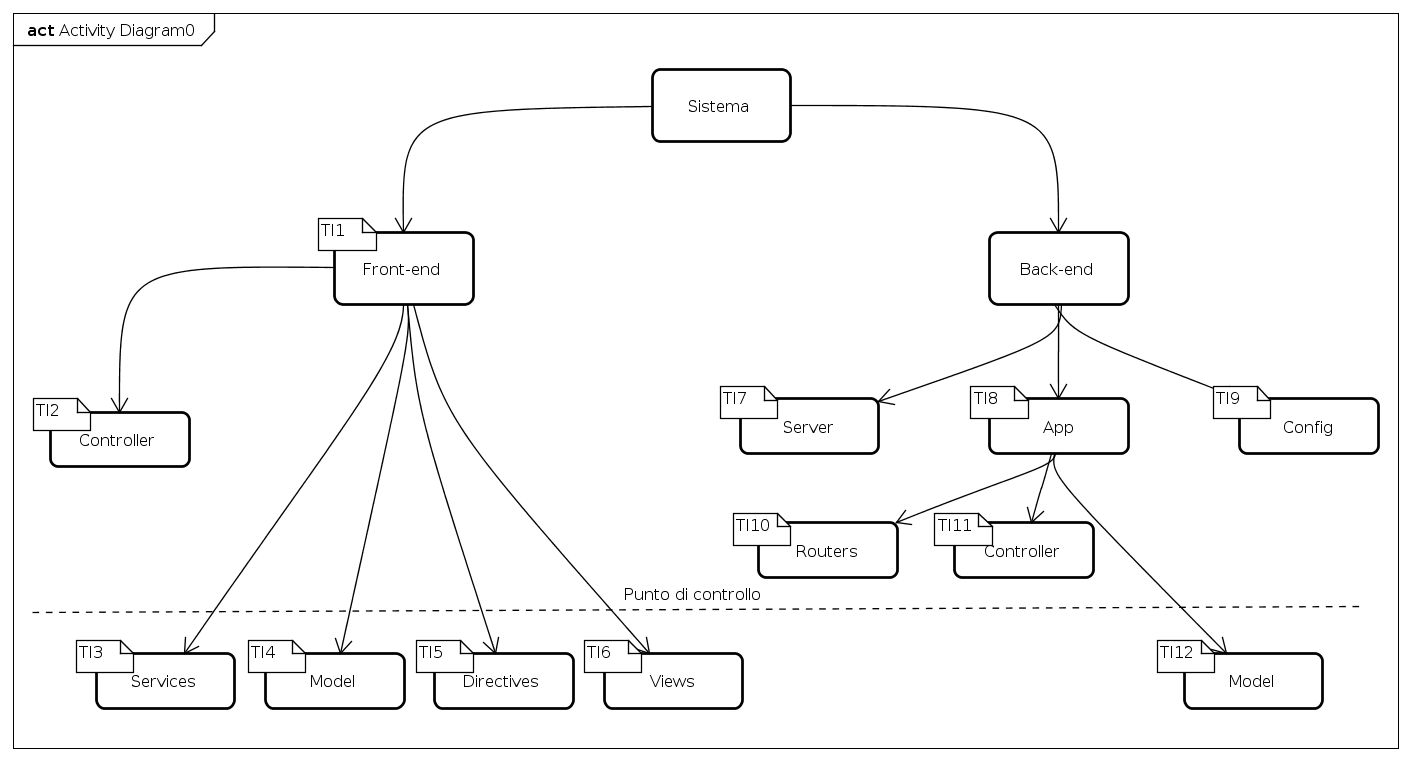
\includegraphics[scale=0.45]{AlberoDiIntegrazione.png}
	\caption{Albero di integrazione delle componenti}
\end{figure}
\FloatBarrier

Nell'approccio top-down dei test di integrazione i moduli di livello più alto vengono sottoposti a test e integrati per primi. Così facendo anche la logica di alto livello e il flusso di dati vengono sottoposti a test fin da subito; sarà perciò necessario simulare le componenti di livello più basso con degli stub. Una volta codificate, le componenti di più basso livello dovranno a loro volta essere integrate e testate. L'approccio top-down rientra tra le strategie di integrazione incrementali, che conferiscono il vantaggio di poter determinare in modo più immediato quale componente causa problemi: i difetti rilevati dai test, infatti, nella maggioranza dei casi saranno da attribuirsi all'ultima componente aggiunta.
\begin{figure}[ht]
	\centering
	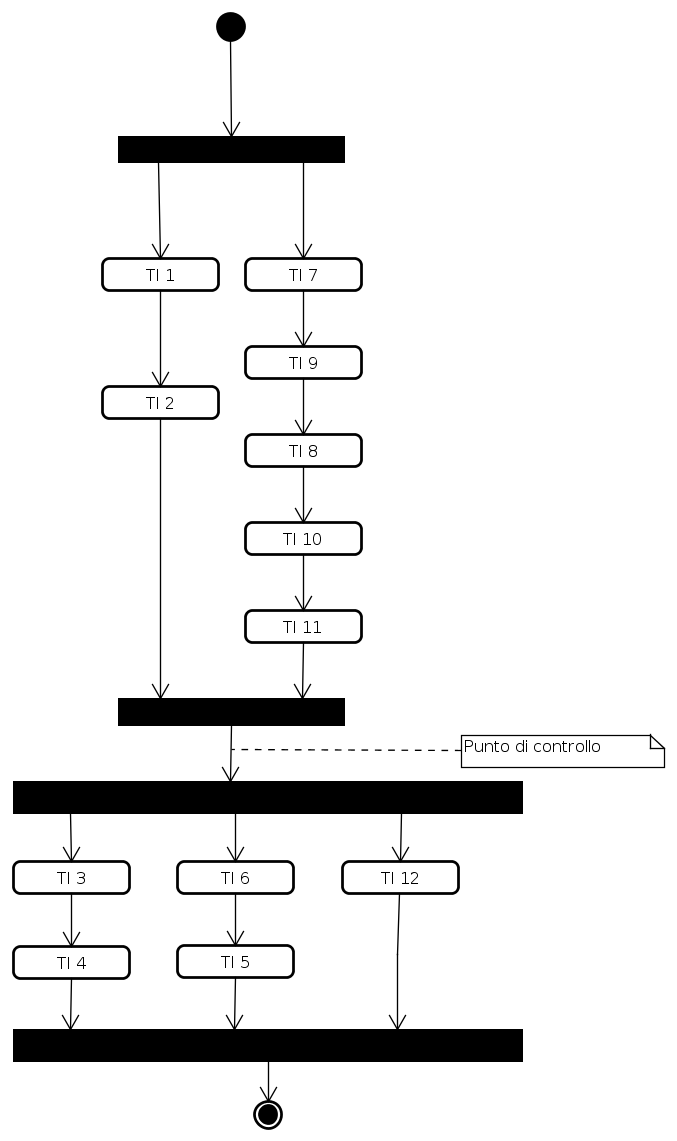
\includegraphics[scale=0.45]{DiagrammaDiAttivita.png}
	\caption{Diagramma di attività dei test di integrazione}
\end{figure}
\FloatBarrier

% TABELLA
\normalsize
\begin{longtable}[ht]{|c|>{}m{10cm}|c|}
\hline 
\textbf{Id Test} & \textbf{Descrizione} & \textbf{Stato}\\
\hline
\endhead
\hypertarget{TI1}{TI1} & Viene verificato che l’applicazione Web gestisca
correttamente il Front-End del prodotto e le sue interazioni
con il Back-End. & \textit{Non Implementato}\\ \hline
\hypertarget{TI2}{TI2} & Viene verificato che i Controllers del Front-End si integrino
correttamente nell’applicazione Web. & \textit{Non Implementato}\\ \hline
\hypertarget{TI3}{TI3} & Viene verificato che i Services permettano di interagire
correttamente con il Back-End. & \textit{Non Implementato}\\ \hline
\hypertarget{TI4}{TI4} & Viene verificato che il Model si integri correttamente con i
Services e con le componenti dell’applicazione che lo
utilizzano. & \textit{Non Implementato}\\ \hline
\hypertarget{TI5}{TI5} & Viene verificato che le Directives si integrino correttamente
con le Views. & \textit{Non Implementato}\\ \hline
\hypertarget{TI6}{TI6} & Viene verificato che le Views si integrino correttamente con i
Controllers e che visualizzino in modo corretto i dati da essi
ricevuti. & \textit{Non Implementato}\\ \hline
\hypertarget{TI7}{TI7} & Viene verificato che il server si avvii correttamente,
utilizzando Config per effettuare le configurazioni
dell’applicazione, e che l’applicazione Web gestisca
correttamente il Back-End del prodotto in modo tale da
fornire al Front-End tutte le informazioni richieste. & \textit{Non Implementato}\\ \hline
\hypertarget{TI8}{TI8} & Viene verificato che App si integri correttamente con le
librerie di Node.js utilizzate. & \textit{Non Implementato}\\ \hline
\hypertarget{TI9}{TI9} & Viene verificato che Config si integri con Server, carichi
correttamente tutte le librerie per Node.js che utilizzerà e
che istanzi le classi del package App in modo corretto. & \textit{Non Implementato}\\ \hline
\hypertarget{TI10}{TI10} & Viene verificato che Config si integri con Server, carichi
correttamente tutte le librerie per Node.js che utilizzerà e
che istanzi le classi del package App in modo corretto. & \textit{Non Implementato}\\ \hline
\hypertarget{TI11}{TI11} & Viene verificato che i Controllers si integrino correttamente
e gestiscano le richieste inoltrate dai Routers. & \textit{Non Implementato}\\ \hline
\hypertarget{TI12}{TI12} & Viene verificato che il Model si integri correttamente con i
Controllers per la gestione dell’inserimento, della modifica e
dell’eliminazione dei dati. & \textit{Non Implementato}\\ \hline
\caption[Test di Integrazione]{Test di Integrazione}
\label{tabella:test2}
\end{longtable}
\clearpage